\section{SPIN verification of alley synchronization - Step 2}

Since it can be difficult to visualize/check all possible interleavings between the different car operations, \texttt{SPIN} \cite{spin} is used to help verify the alley synchronization, using the Promela language.

Spin builds the system as a finite state machine and validates a given (or several) predicate on each state as a model checker. More on model checking can be seen in the book \textit{Formal Methods an Appetizer} \cite{formalmethods} section 5.5 from the course 02141 \textit{Computer Science Modelling}.

For the alley synchronization, we wish to verify that no cars in the alley go in different directions, e.g. if a car enters from the bottom, no car should be traveling down the alley.

Translating our synchronization algorithm into Promela needs to be done carefully. Promela has no functions/methods or objects, meaning that the objects must be unravelled and the methods will be defined as inlines. Since the solution uses semaphores, which are defined to work atomically, the semaphore operations are set to be atomic. The inner resources handled by the semaphore has to be declared as exposed variables, but is only used by the semaphore inlines. This way we can simulate the same behaviors in Promela as our \texttt{Java} algorithm for the alley synchronization.

An example of the semaphores as an inline is seen in code snippet \ref{src:sem_pml}.
\begin{lstlisting}[language=promela, caption=Semaphore protocol in Promela, label=src:sem_pml]
inline sInAlleyP(){
atomic {do ::sInAlley==0->skip; ::else->sInAlley--;break; od;}
}
inline sInAlleyV(){
atomic {sInAlley++}
}
\end{lstlisting} 

For the \texttt{V} operation of the semaphore it is not strictly necessary to define the increment operation as atomic, since Promela evaluates all individual statements as atomic, but it is kept in this case to indicate, that it is inteded to be atomic.

The alley methods for \texttt{enter} and \texttt{leave} are also implemented as inliners, but using the semaphores for mutual exclusion instead of defining atomic statements. The \texttt{enter} and \texttt{leave} protocols are shown in code snippet \ref{src:enter_pml} and  \ref{src:leave_pml} for the group entering from the top. A similar protocol exists for the group entering from the bottom.
\begin{figure}[H]
    \begin{multicols}{2}
    \begin{lstlisting}[language=promela, caption=\texttt{enter} protocol, label=src:enter_pml]
    sTopMutexP();
    if :: carsTop == 0 ->
        	sInAlleyP();
       :: else -> skip;
    fi;
    carsTop++;
    sTopMutexV();
    \end{lstlisting} 
    
    \begin{lstlisting}[language=promela, caption=\texttt{leave} protocol, label=src:leave_pml]
    sTopMutexP();
    carsTop--;
    if :: carsTop == 0 ->
        	sInAlleyV();
       :: else -> skip;
    fi;
    sTopMutexV();
    \end{lstlisting}
    \end{multicols}
\end{figure}

Since only the alley synchronization is checked in this section, the cars drive around for an arbitariry amount of steps inside and outside the alley. This simulates their varying speeds when they pass the gates. The car protocols are seen in code snippet \ref{src:car_pml}.
    
    \begin{lstlisting}[language=promela, caption=Cars implemented in Promela, label=src:car_pml]
    active [N] proctype Car()
    {
    do 
    :: /* Run around the loop for indeterminate time*/
       do :: true -> skip :: break od; 
    
       alleyEnter(_pid);
    
       /* Run around the loop for indeterminate time*/
       do :: true -> skip :: break od; 
    
       alleyLeave(_pid);
    od
    }
    \end{lstlisting} 

The safety property we wish to verify in all states, is that \texttt{carsTop} and \texttt{carsBottom} is not positive (non-zero) at the same time. If they both contained a positive value, it would mean that cars have entered from both sides of the alley and the directions are therefore not mutually excluded.

This can be formally stated as:
\begin{gather*}
    \texttt{mutex} \triangleq \forall \square \left( \texttt{carsTop} = 0 \; \vee \; \texttt{carsBottom} = 0 \right) 
\end{gather*}
The formula is read as "For all reachable states, either \texttt{carsTop} or \texttt{carsBottom} is zero", which is exactly what we want.

This can be expressed in Promela as:
\begin{gather*}
    \texttt{ltl mutex\{[](carsTop==0||carsBottom==0)\} }
\end{gather*}

Further liveness properties such as \textit{obligingness} and \textit{resolution}, are also checked as no car should wait unnecessarily (accept the case with car 1 and 2 as stated in the assignment), and no deadlock should occur. These are defined in Promela as:
\begin{gather*}
    \texttt{
    ltl obl\{[]((Car[0]@enter\&\&[](!Car[1]@enter))-><>(Car[0]@inside))\}
    } \\
    \texttt{
    ltl res\{[](Car[0]@enter\&\&Car[N]@enter-><>(Car[0]@inside||Car[N]@inside))\}
    }
\end{gather*}

Notice that \texttt{Car[0]} and \texttt{Car[N]} are chosen in the in the liveness properties to represent each group of cars, where \texttt{Car[0]} and \texttt{Car[1]} are representing two cars from the same group.

The solution is not fair. This is easily seen, if the amount of cars is high. The cars in the alley may not necessarily leave before the another car from the same group enters. This is especially seen if \textbf{slowdown} is applied to the alley. Hence the obligingness property is not  \texttt{Car[0]} and \texttt{Car[N]}, as the rest of the \texttt{Car[N]}'s group could cause starvation for \texttt{Car[0]}.

The safety property is satisfied in all reachable states, as seen in figure \ref{fig:spinvalidation}. Likewise for the liveness properties, although search depth is far deeper, as \textit{breadth first search} is not used for acceptance verification.

\begin{figure}[H]
    \centering
    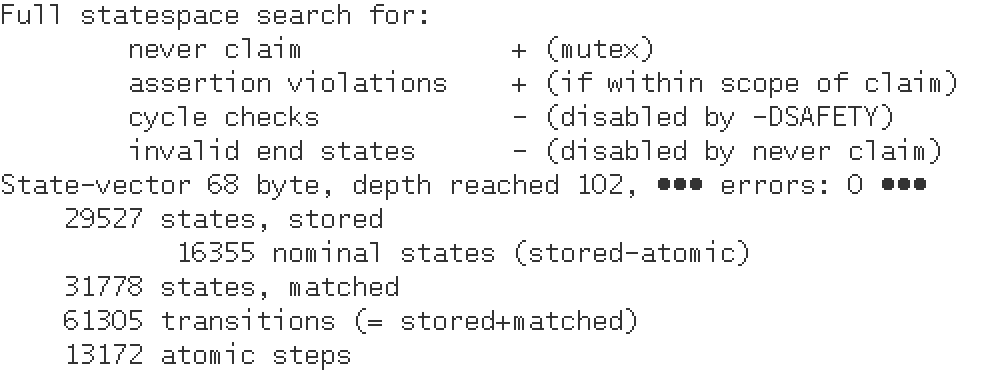
\includegraphics[width=0.7\textwidth]{fig/spinverification.png}
    \caption{Result for \texttt{mutex} safety property from SPIN}
    \label{fig:spinvalidation}
\end{figure}